\documentclass{article}
\usepackage{amsmath}
\usepackage{amssymb}
\usepackage[margin=1cm,footskip=0.25cm]{geometry}
\usepackage{graphicx}
\usepackage{float}
\usepackage{multirow} % Added for multirow cells in tables
\usepackage{adjustbox} % Added for resizing tables


\begin{document}
\begin{center}
\textbf{\LARGE Lineare Algebra}
\end{center}

\section*{Matrizen}
\begin{minipage}[t]{0.45\textwidth}
    \begin{align*}
        A &= \begin{pmatrix}
        1 & 2 & 3 \\
        4 & 5 & 6 \\
        7 & 8 & 9
        \end{pmatrix}, \quad
        B = \begin{pmatrix}
        2 & 3 & 4 \\
        5 & 6 & 7 \\
        8 & 9 & 10
        \end{pmatrix}
    \end{align*}
    \subsubsection*{Addition und Subtraktion}
    \begin{align*}
    A + B &= \begin{pmatrix}
    3 & 5 & 7 \\
    9 & 11 & 13 \\
    12 & 14 & 16
    \end{pmatrix}, \quad
    A - B = \begin{pmatrix}
    -1 & -1 & -1 \\
    -1 & -1 & -1 \\
    -1 & -1 & -1
    \end{pmatrix}
    \end{align*}

    \subsubsection*{Matrizenmultiplikation}
    \begin{figure}[H]
        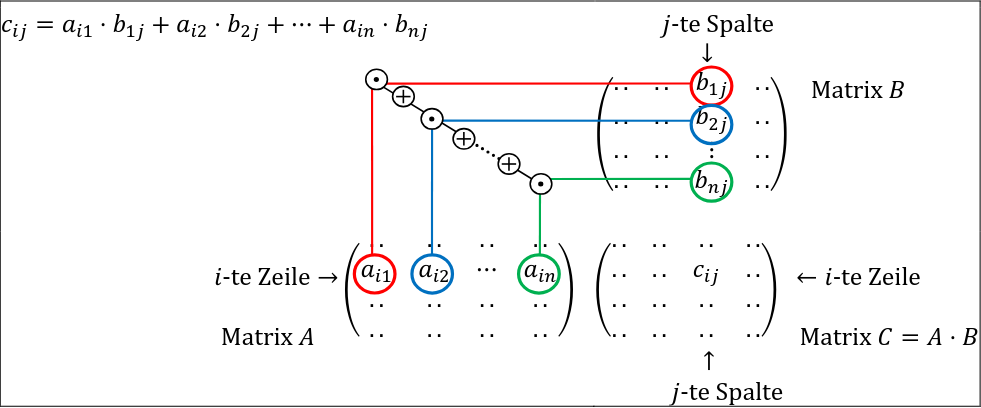
\includegraphics[scale=0.2]{images/matrixmult.png}
    \end{figure}
\end{minipage}
\hfill
\begin{minipage}[t]{0.45\textwidth}
    \subsubsection*{Transponierte Matrix}
    \begin{align*}
    A^T &= \begin{pmatrix}
    1 & 4 & 7 \\
    2 & 5 & 8 \\
    3 & 6 & 9
    \end{pmatrix}
    \end{align*}

    \subsubsection*{Multiplikation mit Skalar}
    \begin{align*}
    cA &= 2 \cdot A = \begin{pmatrix}
    2 & 4 & 6 \\
    8 & 10 & 12 \\
    14 & 16 & 18
    \end{pmatrix}
    \end{align*}
\end{minipage}

\section*{Lineare Gleichungssysteme}
\begin{minipage}[t]{0.45\textwidth}
    \subsection*{Zeilenstufenform}
    Die Matrix ist in Zeilenstufenform, wenn:
    \begin{itemize}
        \item Alle Zeilen, die nur Nullen enthalten, stehen am Ende der Matrix.
        \item Die erste Nicht-Null-Zahl in jeder Zeile (der sogenannte Pivot) ist 1 (führende Eins).
        \item Der Pivot jeder Zeile steht weiter rechts als der Pivot der vorherigen Zeile.
    \end{itemize}
    Reduzierte Zeilenstufenform (RREF) ist erreicht, wenn:
    \begin{itemize}
        \item Jede Spalte, die eine führende Eins enthält, hat nur Nullen in allen anderen Zeilen.
    \end{itemize}    
\end{minipage}
\hfill
\begin{minipage}[t]{0.45\textwidth}
    \subsection*{Parameterdarstellung}
    \subsubsection*{führende Unbekannte}
    Die führenden Unbekannten sind die Variablen, die in der Zeilenstufenform der Matrix als Pivot-Elemente auftreten. Sie sind eindeutig bestimmt und können direkt aus den Gleichungen abgelesen werden.
    \subsubsection*{freie Unbekannte}
    Die freien Unbekannten sind die Variablen, die nicht als Pivot-Elemente auftreten. Sie können beliebige Werte annehmen.
    
\end{minipage}
\subsubsection*{Beispiel}
\begin{align*}
    \begin{pmatrix}
    1 & -2 & 0 & 3 | 5 \\
    0 & 0 & 1 & 1 | 3
    \end{pmatrix}
\end{align*}
In diesem Beispiel sind $x_1$ und $x_3$ die führenden Unbekannten, während $x_2$ und $x_34$ freie Unbekannte sind. Die Lösung kann in Parameterform dargestellt werden:

\begin{minipage}[t]{0.45\textwidth}
    \begin{align*}
        x_2 &= \lambda \quad (\lambda \in \mathbb{R}) \\
        x_4 &= \mu \quad (\mu \in \mathbb{R})
    \end{align*}
    Erste Zeile: \( x_1 - 2x_2 + 3x_4 = 5 \), daraus \( x_1 = 5 + 2\lambda - 3\mu \)\\
    Zweite Zeile: \( x_3 + x_4 = 3 \), daraus \( x_3 = 3 - \mu \)
\end{minipage}
\hfill
\begin{minipage}[t]{0.45\textwidth}
    In Vektorform:

    \begin{align*}
        \begin{pmatrix}
        x_1 \\
        x_2 \\
        x_3 \\
        x_4
        \end{pmatrix}
        = 
        \begin{pmatrix}
        5 \\
        0 \\
        3 \\
        0
        \end{pmatrix}
        + \lambda
        \begin{pmatrix}
        2 \\
        1 \\
        0 \\
        0
        \end{pmatrix}
        + \mu
        \begin{pmatrix}
            -3 \\
            0 \\
            -1 \\
            1
        \end{pmatrix}
    \end{align*}
\end{minipage}

\section*{Lösbarkeit von LGS}
\begin{itemize}
    \item \textbf{Eindeutige Lösung:} Wenn die Matrix in Zeilenstufenform keine freien Unbekannten hat. (rg(A) = Anzahl der Unbekannten (n))
    \item \textbf{Unendlich viele Lösungen:} Wenn die Matrix in Zeilenstufenform mindestens eine freie Unbekannte hat. ($rg(A) <  n$)
    \item \textbf{Keine Lösung:} Wenn die Matrix in Zeilenstufenform eine Zeile der Form \(0 = c\) (mit \(c \neq 0\)) enthält. ($rg(A) \neq rg(A|\vec{c})$)
\end{itemize}

\section*{Vektorgeometrie}
\begin{minipage}[t]{0.45\textwidth}
    \subsection*{Einheitsvektor}
    Ein Einheitsvektor ist ein Vektor mit der Länge/Betrag 1.

    \subsection*{Koliniare Vektoren}
    Zwei Vektoren \( \vec{a} \) und \( \vec{b} \) sind kolinear, wenn sie in die gleiche Richtung zeigen oder entgegengesetzt sind, bzw. das Vektorprodukt 0 ergibt. Mathematisch ausgedrückt: \( \vec{a} = k \cdot \vec{b} \) für ein Skalar \( k \).
    Der Nullvektor ist kolinear zu jedem Vektor. \( \vec{a} \times \vec{b} = \vec{0} \)

    \subsection*{Komplanare Vektoren}
    Drei Vektoren \( \vec{a}, \vec{b}, \vec{c} \) sind komplanar, wenn sie in einer Ebene liegen. Dies ist der Fall, wenn das Skalarprodukt der Kreuzprodukte Null ist: \( \vec{a} \times \vec{b} \cdot \vec{c} = 0 \).

    \subsection*{Orthogonale Projektion}
    Die orthogonale Projektion eines Vektors \( \vec{a} \) auf einen Vektor \( \vec{b} \) wird berechnet als:
    \begin{equation*}
        \vec{b}_{\vec{a}} = \frac{\vec{a} \cdot \vec{b}}{|\vec{a}|^2} \cdot \vec{a} 
        \quad \Leftrightarrow \quad 
        |\vec{b}_{\vec{a}}| = \frac{|\vec{a} \cdot \vec{b}|}{|\vec{a}|}
    \end{equation*}
    Die Projektion gibt den Anteil von \( \vec{a} \) in Richtung von \( \vec{b} \) an.

    \subsection*{Vektorprodukt}
    Das Vektorprodukt (Kreuzprodukt) zweier Vektoren \( \vec{a} = (a_1, a_2, a_3) \) und \( \vec{b} = (b_1, b_2, b_3) \) wird berechnet als:
    \begin{equation*}
    \vec{a} \times \vec{b} = 
    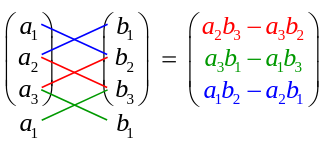
\includegraphics[scale=0.3]{images/vektorprodukt.png}
    \end{equation*}
    \begin{equation*}
        |\vec{a} \times \vec{b}| = |\vec{a}| \cdot |\vec{b}| \cdot \sin(\theta)
    \end{equation*}
    Das Vektorprodukt ist ein Vektor, der orthogonal zu beiden Ausgangsvektoren steht. Die Länge des Vektorprodukts entspricht der Fläche des Parallelogramms, das von den beiden Vektoren aufgespannt wird.

    \subsubsection*{Eigenschaften des Vektorprodukts}
    \begin{itemize}
        \item \( \vec{a} \times \vec{b} = -(\vec{b} \times \vec{a}) \) (Antisymmetrie)
        \item Distributivität: \( \vec{a} \times (\vec{b} + \vec{c}) = \vec{a} \times \vec{b} + \vec{a} \times \vec{c} \)
        \item Gemischtes Assoziativ-Gesetz: \( \lambda \cdot (\vec{a} \times \vec{b}) = (\lambda \cdot \vec{a}) \times \vec{b} = \vec{a} \times (\lambda \cdot \vec{b}) \)
    \end{itemize}
\end{minipage}
\hfill
\begin{minipage}[t]{0.45\textwidth}
    \subsection*{Betrag eines Vektors}
    Der Betrag eines Vektors \( \vec{a} = (a_1, a_2, a_3) \) wird berechnet als:
    \begin{equation*}
        |\vec{a}| = \sqrt{a_1^2 + a_2^2 + a_3^2}
    \end{equation*}


    \subsection*{Basisvektoren}
    Eine Basis eines Vektorraums ist eine Menge von Vektoren, die linear unabhängig sind und den gesamten Raum aufspannen. Jeder Vektor im Raum kann als Linearkombination dieser Basisvektoren dargestellt werden.
    
    \subsection*{Skalarprodukt}
    Das Skalarprodukt zweier Vektoren \( \vec{a} = (a_1, a_2, a_3) \) und \( \vec{b} = (b_1, b_2, b_3) \) wird berechnet als:
    \begin{equation*}
        \vec{a} \cdot \vec{b} = a_1 b_1 + a_2 b_2 + a_3 b_3
    \end{equation*}
    Das Skalarprodukt ist ein Maß für die Ähnlichkeit zweier Vektoren. Es ist null, wenn die Vektoren orthogonal zueinander sind.
    \subsection*{Winkel zwischen Vektoren}
    Der Winkel \( \theta \) zwischen zwei Vektoren \( \vec{a} \) und \( \vec{b} \) kann mit dem Skalarprodukt berechnet werden:
    \begin{equation*}
        \cos(\theta) = \frac{\vec{a} \cdot \vec{b}}{|\vec{a}| |\vec{b}|} 
        \quad \Leftrightarrow \quad 
        \theta = \arccos\left(\frac{\vec{a} \cdot \vec{b}}{|\vec{a}| |\vec{b}|}\right) 
    \end{equation*}

    \subsection*{Gegenseitige Lage von Geraden im Raum}
    \begin{center}
    \resizebox{\textwidth}{!}{%
    \begin{tabular}{|l|l|l|l|}
    \hline
    \multicolumn{2}{|c|}{} & \multicolumn{2}{c|}{Gibt es einen gemeinsamen Punkt?} \\
    \cline{3-4}
    \multicolumn{2}{|c|}{} & ja & nein \\
    \hline
    \multirow{2}{*}{Sind die Richtungsvektoren kollinear?} & ja & identisch & echt parallel \\
    \cline{2-4}
    & nein & schneidend & windschief \\
    \hline
    \end{tabular}%
    }
    \end{center}
    \subsection*{Abstand zwischen einer Geraden und einem Punkt}
    Der Abstand \( d \) zwischen einer Geraden \( g \) und einem Punkt \( P \) kann mithilfe der Fläche des Parallelogramms berechnet werden, 
    das von den Richtungsvektoren der Geraden und dem Vektor vom Punkt auf die Gerade aufgespannt wird:
    \begin{equation*}
        \overrightarrow{PA} = \vec{P} - \vec{A}
    \end{equation*}
    \begin{equation*}
        F = |\overrightarrow{PA} \times \vec{a}|
        \quad \text{(Fläche des Parallelogramms)}
    \end{equation*}
    \begin{equation*}
        l = \frac{F}{|\vec{a}|}
        \quad \text{(Länge der Geraden)}
    \end{equation*}
\end{minipage}

\begin{minipage}[t]{0.45\textwidth}
    \subsection*{Koordinatendarstellung von Geraden in der Ebene}
    Eine Gerade in der Ebene kann durch die Gleichung
    \begin{equation*}
        g: ax + by + c = 0
    \end{equation*}
    dargestellt werden.
    \subsubsection*{Umrechnung Parameterdarstellung $\to$ Koordinatendarstellung}
    \begin{equation*}
        \vec{r}(A) = \begin{pmatrix}
        x \\
        y
        \end{pmatrix} = \vec{r}(P) + \lambda \cdot \vec{a}
    \end{equation*}
    Daraus lässt sich ein Gleichungssystem ableiten
\end{minipage}
\hfill
\begin{minipage}[t]{0.45\textwidth}
    \subsubsection*{Umrechnung Koordinatendarstellung $\to$ Parameterdarstellung}
    Wir bestimmen zwei beliebige Punkte auf $g$, indem wir die $x$-Koordinaten frei wählen und die
zugehörigen $y$-Koordinaten aus der Koordinatendarstellung von $g$ berechnen. Aus diesen beiden
Punkten können wir dann eine Parameterdarstellung von $g$ gewinnen.
\end{minipage}

\section*{Ebenen}
\begin{minipage}[t]{0.45\textwidth}
    \subsection*{Parameterdarstellung}
    Eine Ebene im Raum kann durch die Gleichung
    \begin{equation*}
        E: \vec{r}(P) + \lambda_1 \cdot \vec{a} + \lambda_2 \cdot \vec{b}
    \end{equation*}
    dargestellt werden, wobei \( \vec{r}(P) \) ein Punkt auf der Ebene ist und \( \vec{a} \) und \( \vec{b} \) zwei Richtungsvektoren der Ebene sind.
    \subsection*{Koordinatendarstellung}
    Eine Ebene kann auch in der Koordinatendarstellung angegeben werden:
    \begin{equation*}
        E: ax + by + cz + d = 0
    \end{equation*}
    Hierbei sind \( a, b, c \) die Komponenten des Normalenvektors der Ebene und \( d \) eine Konstante.

    \subsection*{Abstand zwischen einer Ebene und einem Punkt}
    Um den Abstand $l$ zu berechnen, gehen wir folgendermassen vor:
    Wir wählen einen beliebigen Punkt $P$ der Ebene $E$ (rechts "im
    Profil" abgebildet). Dann projizieren wir den Verbindungsvektor
    $\overrightarrow{PA}$ auf den Normalenvektor $\vec{n}$ der Ebene. Die Länge dieser
    Projektion ist gerade der gesuchte Abstand $l$.
    \begin{equation*}
        l = \frac{|ax_A + by_A + cz_A + d|}{|\vec{n}|}
    \end{equation*}
\end{minipage}
\hfill
\begin{minipage}[t]{0.45\textwidth}
    \subsection*{Schnittpunkt Ebene und Gerade}
    Der Schnittpunkt einer Ebene \( E \) und einer Geraden \( g \) kann mithilfe eines LGS gefunden werden. 
    \begin{equation*}
        E: \begin{pmatrix}
            1 \\
            0 \\
            -2
        \end{pmatrix} + \lambda \cdot \begin{pmatrix}
            3 \\
            -2 \\
            1
        \end{pmatrix} + \mu \cdot \begin{pmatrix}
            0 \\
            4 \\
            3
        \end{pmatrix}
    \end{equation*}
    \begin{equation*}
        g: \begin{pmatrix}
            1 \\
            -3 \\
            -4
            \end{pmatrix} + v \cdot \begin{pmatrix}
                -2 \\
                1 \\
                -1
            \end{pmatrix}
    \end{equation*}
    Um den Schnittpunkt zu finden, setzen wir die Ebene und die Gerade gleich und lösen das entstehende LGS

    \subsection*{Gegenseitige Lage von Ebenen}
    \subsubsection*{identisch}
    Zwei Ebenen sind identisch, wenn sie die gleiche Normalenvektor und den gleichen Stützpunkt haben.

    \subsubsection*{echt parallel}
    Zwei Ebenen sind echt parallel, wenn ihre Normalenvektoren kollinear sind, aber sie nicht identisch sind.
    
    \subsubsection*{schneidend}
    In allen anderen Fällen schneiden sich die Ebenen. Der Schnittpunkt kann durch das Lösen eines LGS gefunden werden.
\end{minipage}
\end{document}